% Maxwell-Spannungstensor: Kraft pro Fläche T.n = eps0/2 E^2 (cos 2theta n + sin 2theta t)
% E halbiert den Winkel zwischen n und T.n.
% Gemeinsamer Stil für alle Abbildungen (TikZ -> SVG, siehe figures/build.mjs).
%
% Farben sind Platzhalter ("Sentinels"): build.mjs ersetzt sie im SVG durch
% CSS-Variablen, damit die Abbildungen im hellen und dunklen Modus passen.
% Andere Farben (auch schwarz/weiß) bricht der Build mit Fehler ab.
%
%   fg    Linien, Beschriftung          -> --dark
%   mu    Hilfslinien, Achsen, Maße      -> --gray
%   acc   das eine Konzept der Abbildung -> --secondary (Lime/Oliv)
%   blue  zweite Größe, negative Ladung  -> --fig-blue
%   warm  dritte Größe, positive Ladung  -> --fig-warm
%   bg    Seitenhintergrund (Aussparen)  -> --light
%
% Kein \clip verwenden: pdftocairo macht daraus Clip-Gruppen, in denen exakt
% waagerechte/senkrechte Linien verschwinden. Berechnete Kurven schneidet
% gen/*.py selbst am Rahmen ab.
\documentclass[tikz,border=3pt]{standalone}
\usepackage{amsmath,amssymb,bm}
% Text serifenlos wie die Seite, Mathe in Computer Modern wie KaTeX
\renewcommand{\familydefault}{\sfdefault}
\usetikzlibrary{arrows.meta,calc,decorations.markings,patterns,3d,positioning,angles,quotes}

\definecolor{fg}{RGB}{1,2,3}
\definecolor{mu}{RGB}{4,5,6}
\definecolor{acc}{RGB}{7,8,9}
\definecolor{blue}{RGB}{10,11,12}
\definecolor{warm}{RGB}{13,14,15}
\definecolor{bg}{RGB}{16,17,18}

% Vektoren wie auf der Website (KaTeX \mathbf)
\newcommand{\vv}[1]{\mathbf{#1}}

\tikzset{
  every picture/.style={fg, line width=0.8pt, line cap=round, line join=round,
    >={Stealth[length=5.5pt,width=4.4pt]}},
  every node/.style={font=\small},
  % Linientypen
  main/.style={line width=0.9pt},
  thin/.style={line width=0.5pt},
  aux/.style={mu, line width=0.5pt, dash pattern=on 2.5pt off 2pt},
  axis/.style={mu, line width=0.6pt, ->},
  vec/.style={line width=1.1pt, ->},
  field/.style={line width=0.7pt, postaction={decorate},
    decoration={markings, mark=at position #1 with {\arrow{Stealth[length=4.5pt,width=3.6pt]}}}},
  field/.default=0.5,
  % Flächen
  soft/.style={fill=#1, fill opacity=0.14},
  soft/.default=acc,
  % Ladungen
  qpos/.style={circle, fill=warm, inner sep=0pt, minimum size=9pt,
    path picture={\draw[bg, line width=0.9pt] ($(path picture bounding box.center)+(-2pt,0)$) -- +(4pt,0)
      ($(path picture bounding box.center)+(0,-2pt)$) -- +(0,4pt);}},
  qneg/.style={circle, fill=blue, inner sep=0pt, minimum size=9pt,
    path picture={\draw[bg, line width=0.9pt] ($(path picture bounding box.center)+(-2pt,0)$) -- +(4pt,0);}},
  dot/.style={circle, fill=fg, inner sep=0pt, minimum size=3pt},
  % Beschriftung mit Aussparung, damit Linien den Text nicht kreuzen
  lbl/.style={fill=bg, inner sep=1.5pt},
  % Icons: kräftigere Linien, keine Schrift
  icon/.style={line width=1.6pt, >={Stealth[length=6pt,width=5pt]}},
}

\begin{document}
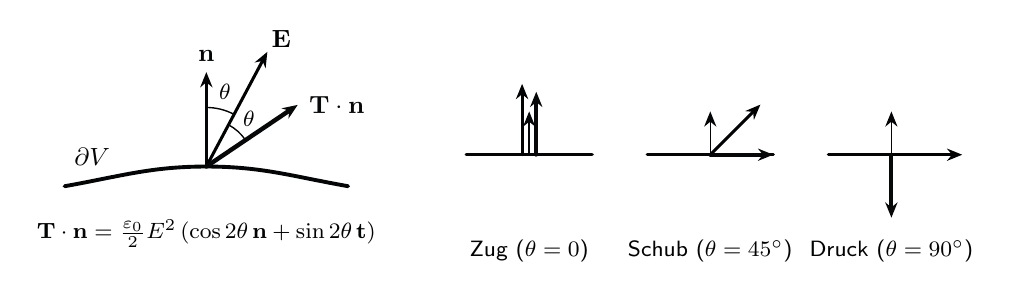
\begin{tikzpicture}
  % ---------- allgemeiner Fall ----------
  \def\th{28}
  \draw[mu, line width=1.4pt] (-1.8,-0.25) to[out=10, in=180] (0,0) to[out=0, in=170] (1.8,-0.25);
  \node[mu, anchor=south] at (-1.45,-0.12) {$\partial V$};
  \coordinate (O) at (0,0);
  \draw[vec, mu] (O) -- (0,1.2) node[anchor=south, text=mu] {$\vv n$};
  \draw[vec] (O) -- (90-\th:1.65) node[anchor=south west, inner sep=1pt] {$\vv E$};
  \draw[vec, acc, line width=1.6pt] (O) -- (90-2*\th:1.4) node[anchor=west] {$\mathbf T\cdot\vv n$};
  \coordinate (N) at (0,1); \coordinate (Ev) at (90-\th:1); \coordinate (F) at (90-2*\th:1);
  \pic[draw, mu, thin, angle radius=0.75cm, "$\theta$"{font=\footnotesize, text=mu}, angle eccentricity=1.3] {angle = Ev--O--N};
  \pic[draw, mu, thin, angle radius=0.6cm, "$\theta$"{font=\footnotesize, text=mu}, angle eccentricity=1.35] {angle = F--O--Ev};
  \node[anchor=north, font=\footnotesize] at (0,-0.55) {$\mathbf T\cdot\vv n=\tfrac{\varepsilon_0}{2}E^2\,(\cos 2\theta\,\vv n+\sin 2\theta\,\vv t)$};
  % ---------- Grenzfälle ----------
  \foreach \k/\t/\txt in {0/0/{Zug ($\theta=0$)}, 1/45/{Schub ($\theta=45^\circ$)}, 2/90/{Druck ($\theta=90^\circ$)}} {
    \begin{scope}[xshift={4.1cm+\k*2.3cm}, yshift=0.15cm]
      \draw[mu, line width=1.2pt] (-0.8,0) -- (0.8,0);
      \draw[vec, mu, thin] (0,0) -- (0,0.55);
      \ifnum\t=0
        \draw[vec] (-0.09,0) -- ++(0,0.9);
        \draw[vec, acc, line width=1.4pt] (0.09,0) -- ++(0,0.8);
      \else
        \draw[vec] (0,0) -- (90-\t:0.9);
        \draw[vec, acc, line width=1.4pt] (0,0) -- (90-2*\t:0.8);
      \fi
      \node[font=\footnotesize, anchor=north] at (0,-0.95) {\txt};
    \end{scope}
  }
\end{tikzpicture}
\end{document}
